\documentclass[10pt,oneside,onecolumn,letterpaper]{article}
\usepackage{graphicx}
\usepackage{xcolor}
\usepackage[hidelinks]{hyperref}
\usepackage{booktabs}
\usepackage{adjustbox}

\usepackage[top=.5in, bottom=1in, left=.5in, right=.7in]{geometry}

\usepackage{fontspec}
\setmainfont{Arial}

\begin{document}

%%
% THIS IS THE HEADER
%%
\noindent\colorbox{black}{
\begin{minipage}[c]{.99\linewidth}
  \vspace{.4cm}
  \Large{\color{white}{\textbf{\hspace{.3cm}University of Massachusetts Boston}}}
  \begin{flushright}
    \vspace{-1.2cm}
    
\includegraphics[width=3cm]{gfx/cs460.png}
  \end{flushright}
\end{minipage}
}

%%
% CONTENT STARTS HERE
%%

\vspace{.5cm} % add some space

\noindent\textbf{CS460 Fall 2019} \\
\textbf{Name:} Jared Barresi \\
\textbf{Student ID:} 00974358 \\
\textbf{Due Date:} 09/09/2019

\section*{Assignment 1: Intro}

\textbf{Describe your favorite WebGL demo.}

\vspace{.5cm} % add some space

\noindent My favorite demo is .... (\url{http://madebyevan.com/webgl-water/}). 

\vspace{.5cm}

\noindent The authors do a great job implementing a realistic looking physics simulation, that also has a simple-to-use interface for user interaction. Fluid physics/simulation has always been something of great interest to me, so this example is of great interest (I was originally getting a B.S in Physics at UMB, switched only 2 semesters ago).

\vspace{.5cm} % add some space
\noindent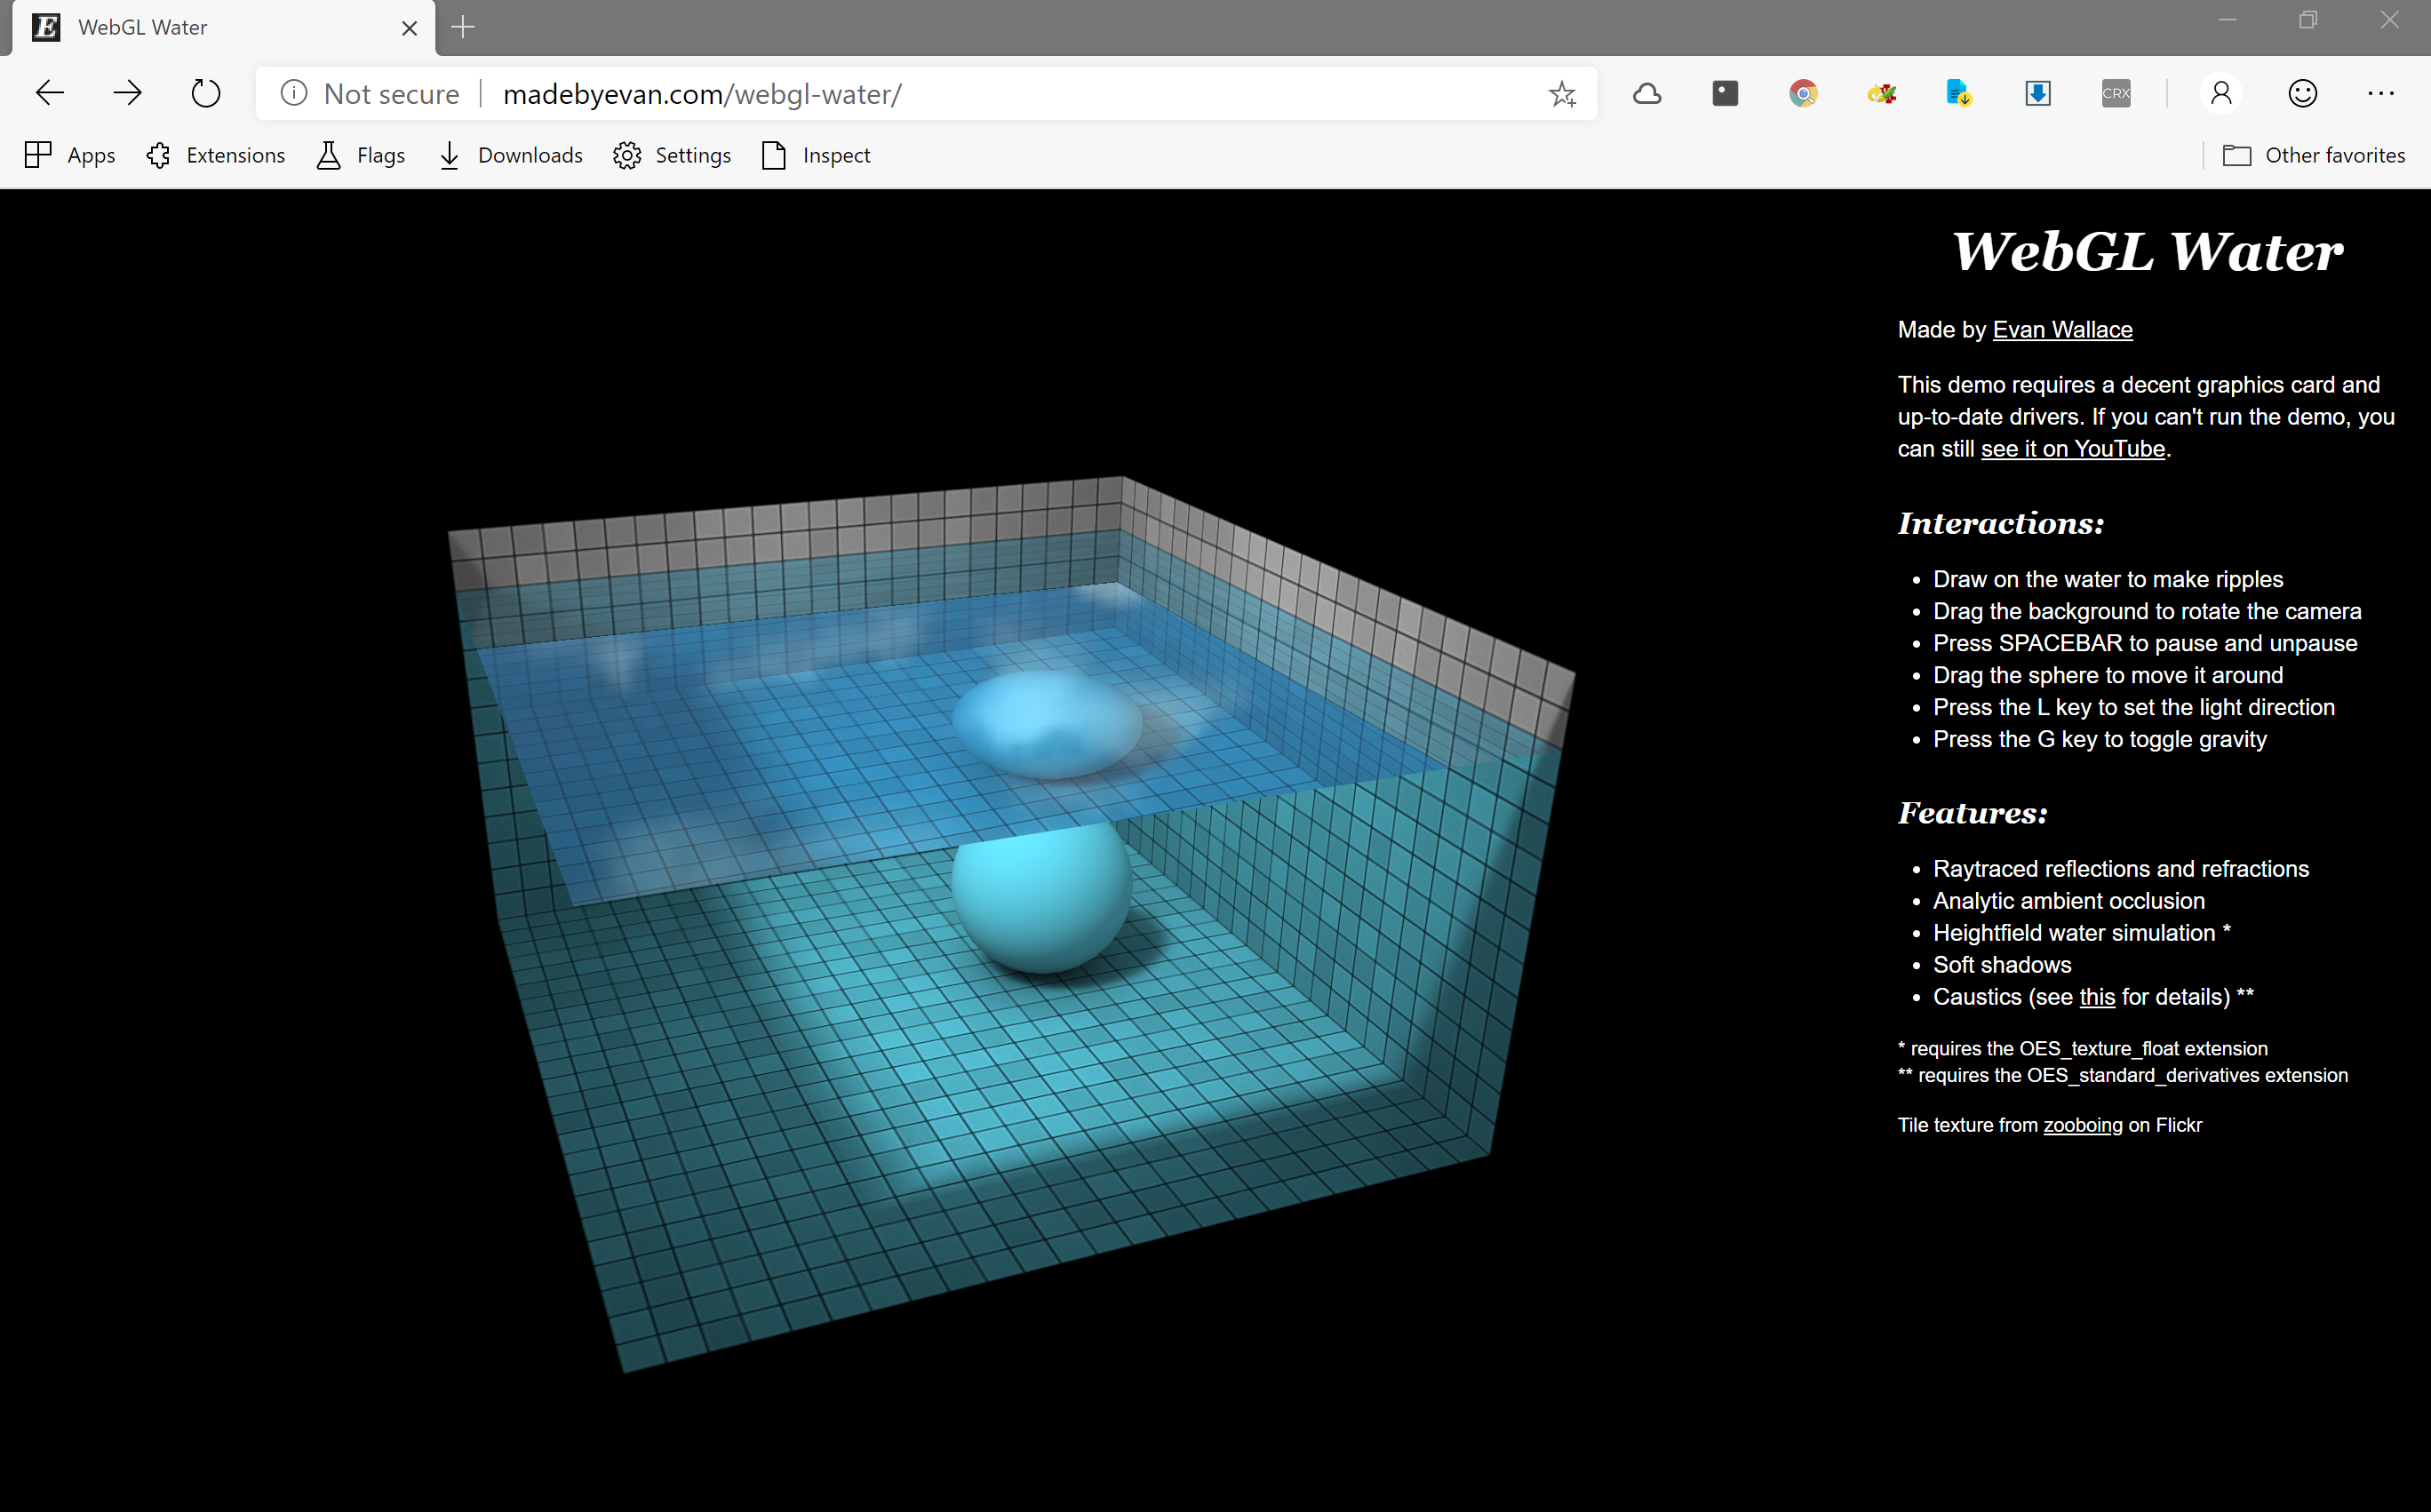
\includegraphics[width=\textwidth]{gfx/full-screenshot-madebyevan_webgl_water.png}

\vspace{.5cm}
\noindent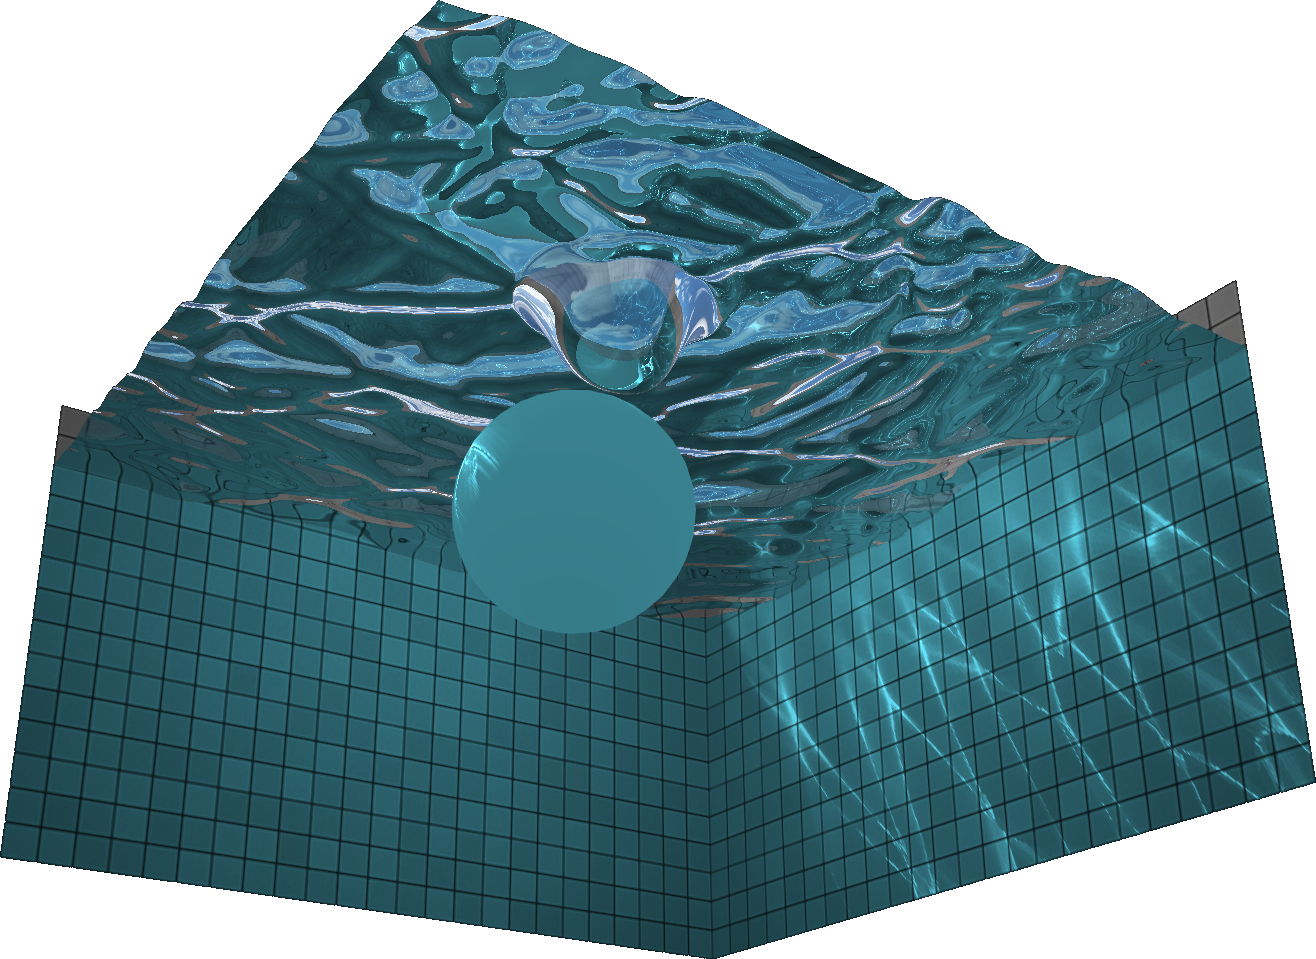
\includegraphics[width=\textwidth]{gfx/screenshot-madebyevan_webgl_water.png}

\vspace{1.0cm}

\noindent\textbf{Technologies used:}

\begin{itemize}
    \item HTML/CSS/JavaScript
    \item Scripts:
    \item Three.js
    \item OES\_texture\_float\_linear-polyfill.js
    \item lightgl.js
    \item cubemap.js
    \item renderer.js
    \item water.js
    \item main.js
\end{itemize}

\noindent\textbf{Bonus:} If possible, try to host the project as your own Github repository and make it accessible via Github pages. Please make sure to credit the original authors. Then, link the repository here: \url{https://ADDLINK}

\end{document}
